\documentclass[english]{article}


\usepackage{graphicx}
\usepackage{times}
\usepackage{pifont}
\usepackage[margin=1in]{geometry}
\usepackage{eurosym}
\usepackage{fancyhdr}
\usepackage[hidelinks]{hyperref}
\usepackage{float}


\pagestyle{fancy}
\fancyhf{}


%HEADER
%**************************************************************************************
\pagestyle{fancy}
\fancyhf{}
%**************************************************************************************
\lhead{Administration}		 	 
\rhead{EFP0700 Database Server} 
\lfoot{EFA12SF}
\cfoot{\thepage}
\rfoot{Nikolay Arsenov\\ Alexey Tukalo}
%**************************************************************************************

\date{}
\setlength\parindent{0pt}

\begin{document}

\title{\vspace{2in}Administration\\
\small for EFP0700 Database Server\\
\vspace{0.5in}
\includegraphics{savonia.jpg}}

\nopagebreak
\maketitle


\vspace{3in}

\author{
\begin{flushright}
Nikolay Arsenov, Alexey Tukalo,\\
EFA12SF,\\
Information Technology,\\
Savonia University of Applied Science
\end{flushright}
}

\date{\today}
\thispagestyle{empty}

\newpage
\setcounter{page}{1}
\setcounter{tocdepth}{2}
\tableofcontents

\newpage

%MAIN CONTENT ******************************************************************************************************************

\section{System Database}
SQL Server system includes five databases: Master, MSDB, Model, Resource, tempdb. Each component is necessary as a tool for the system. \cite{sysdb} Read the description below.
\subsection{Master Database}


Master keeps all records about system-level information for a SQL Server system. This includes instance-wide metadata such as logon accounts, endpoints, linked servers, and system configuration settings. In SQL Server, system objects are no longer stored in the master database; instead, they are stored in the Resource database. Also, master is the database that records the existence of all other databases and the location of those database files and records the initialization information for SQL Server.


\subsection{MSDB Database}

MSDB used by SQL Server Agent for scheduling alerts and jobs, and for recording operators. It also contains history tables, such as the backup and restore history tables. If you want to create a backup to restore your system and create a schedule for that, it will be written by Server Agent tool into the MSDB file. The super user also can see the previous actions and backups using database tool that reads from this file. 


\subsection{Model Database}

The model database is used as the template for all databases created on an instance of SQL Server. Instead of tempdb, the model database always exists on a SQL Server system. The entire contents of the model database, including database options, are copied to the new database. Some of the settings of model are also used for creating a new tempdb during start up.
When a CREATE DATABASE statement is issued, the first part of the database is created by copying in the contents of the model database. The rest of the new database is then filled with empty pages. Also model database used for CREATE TABLE, PROCEDURES and FUNCTIONS, we call the executed template from the model.
If you modify the model database, all databases created after ward will inherit those changes.
\subsection{Resource Database}

The Resource database is a read-only database that contains all the system objects that are included into SQL Server. SQL Server system objects, such as sys.objects, are physically persisted in the Resource database, but they logically appear in the sys schema of every database. The Resource database does not contain user data or user metadata.
In the previous assignment we had to write a function that checks is our table exists in a system, thus we called our resource database, if there were no such table, we create that, and updated our system. The Resource database makes upgrading to a new version of SQL Server an easier and faster procedure.
SQL Server cannot back up the Resource database. You can perform your own file-based or a disk-based backup by treating the mssqlsystemresource.mdf file as if it were a binary (.EXE) file, rather than a database file, but you cannot use SQL Server to restore your backups. Restoring a backup copy of mssqlsystemresource.mdf can only be done manually, and you must be careful not to overwrite the current Resource database with an out-of-date or potentially insecure version.

\subsection{Tempdb Database}

Tempdb – is a workspace for holding temporary or intermediate results (Cach). It created every time an instance of SQL Server, when it started. If the server shuts down, any data in tempdb deletes permanently. Temporary objects in tempdb can be: global or local temporary tables to show up something (for example, the result of merged tables); temporary stored procedures, table variables, or cursors. Also there are objects that are created by the SQL Server Database Engine, for example, work tables to store intermediate results for spools or sorting. AFTER triggers also placed here.
Operations within tempdb are minimally logged. Tempdb is re-created every time SQL Server is started so that the system always starts with a clean copy of the database and rewrites. Temporary tables and stored procedures are dropped automatically on disconnect, no connection and shut down. Therefore, there is never anything in tempdb to be saved from one session to another. Backup and restore operations are not allowed on tempdb.
The size of tempdb can affect the performance of a system. For example, if the tempdb size is too small, the system processing could be too occupied with auto growing the database to support your workload requirement every time that you start SQL Server. You can avoid this overhead by increasing the size of tempdb.
I would like to add, that any user can create temporary object in tempdb, but the certain user can only access their own objects, unless they receive additional permissions.

\section{Disk storage and paging}

\subsection{Content of database}
Every database contains data inside. In case of MS SQL Server the data is stored in tables. In addition database can also store indexes, stored procedures, views, constraints, triggers, functions and transaction log.

\subsubsection{Data Types}
As every other table the database's ones contain columns and rows. The intersection of the elements produces a cell. The data in columns are specified by types. MS SQL Server has different data types:
\begin{itemize}
\item integer
\item float
\item char
\item binary
\item date
\item money
\\\\
And many other more specific types. 
\end{itemize} 
It is also possible to define composite types (UDTs) by user. The UDTs can help you to solve problems very specific for your project.
\subsubsection{Database files}
An SQL Server database is able to contain $2^{60}$ byte of information spread it across $2^{31}$ objects. The main part of the database data is placed in *.mdf files, there are also *.ndf files which are used to store single database across several files, it allows to keep a single database in different file systems. There is also log files with *.ldg extension.

\subsection{Space Allocation}
A database server allocates space by small 8kB sequentially numbered pages. A row can not be stored in several pages and it produces the limit for a row's size, but in case of VARCHAR or VARBINARY it is possible to replace original data by pointer to it. Every page has header. The header tells the database the page number, type, free space, ids of the objects inside. The weight of the header is 96-byte. The pages are the basic I/O unit of the DB, but space is managed thought extents which actually unite 8 pages together.

\subsection{Physical storage}
Every row can be divided into a series of partitions. By default all rows are a single partition, it is possible to change the settings by user. The partition system allows the database to be spread over a computer cluster. Information has binary - tree or heap structure inside a single partition.

\subsection{Buffer management}
Buffer is used to minimize disk I/O. SQL Server uses RAM memory to buffer database pages, the set of pages currently stored in a memory is named a buffer cache. The cache is controlled on a background by the Buffer Manager. A row is placed into the buffer during reading or writing operations and it is saved to a disk only if the cache has not been referenced for sometime. 

\subsection{Concurrency and locking}
Microsoft SQL Server is able to handle concurrent access to data. It can happen when different clients try to read or update same piece of data at the same time. MS developed two concurrency control techniques to prevent any kind of problems at the this kind of situation.
\subsubsection{Pessimistic concurrency}
This type of control is based on locks. Locks can be exclusive or shared. Exclusive lock allows user to have exclusive access to the piece of data. Shared lock provides multiple reading of the data for several clients, but it is not possible to update the date under shared lock. The locks can be set for table, page or even row. The locks are controlled by Lock Manager, it creates new locks and erases useless ones.
\subsubsection{Optimistic concurrency}
An optimistic concurrency control is similar to multiversion one in other databases. Every row is additional identified by the id of the transaction which had created the row, it allows to create new versions of the row during every updates and store all of them at the same time. When the row is processed by update, any other clients will receive old versions of the row, without any locking.

\section{DBCC commands}
\centerline{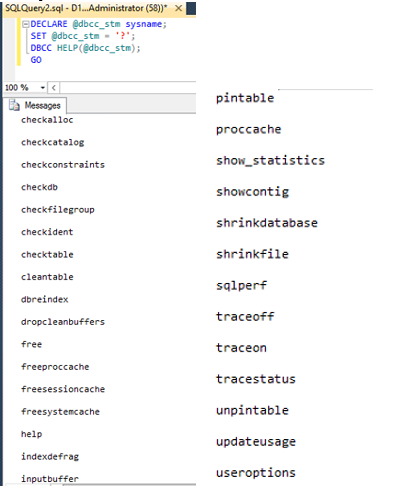
\includegraphics[scale=0.8]{administration/rep/15}}

The Transact-SQL programming language provides DBCC statements that act as Database Console Commands for SQL Server.\\

Database Console Command statements are grouped into the following categories:
\begin{itemize}
\item Maintenance (supporting tasks on a database, index, or file group)
\item Miscellaneous (enable trace flags of removing a DLL from memory)
\item Informational (gather and display various types of information)
\item Validation (valid operations on a database, table, index and etc.)
\end{itemize}

\subsection{Main Console Commands}
A database console command could be run from two variants:
\begin{itemize}
\item the command window 
\item Query analyzer window.
\end{itemize}
DBCC DBREINDEX\\
This statement is used to recreate the indexes for a particular table. This statement rebuilds indexes in a single step. It also assigns fresh pages to reduce internal and external fragmentation.\\\\ 
DBCC DBREPAIR\\
This statement is used to drop or delete a damaged database. However, this command is no longer available with Microsoft SQL Server 2005 and later versions of Microsoft SQL Server. Instead, it has been replaced by the DROP DATABASE Transact-SQL statement. \\\\
DBCC INDEXDEFRAG\\
This statement is used to defragment the clustered and secondary indexes associated with the particular table. The index defragmentation is carried out using the fill factor specified at the time of creation of indexes. While its operation is strikingly similar to that of DBCC DBREINDEX, unlike DBCC INDEXFRAG it does not allow new fill factor to be specified.\\\\ 
DBCC SHRINKDATABASE\\
This statement is used to reduce the size of a database. This statement reduces the physical size of the database log file. An alternate way to shrink a database is to use the commander ALTER DATABASE. \\\\ 
DBCC SHRINKFILE\\
This statement is used to reduce the size of a data file or log file of a particular database. The file could also be shrunk by using the SHRINKFILE attribute of the ALTER DATABASE command. 
\\\\ 
DBCC UPDATEUSAGE\\
This statement is used to correct inaccuracies in the page and row statistics in the views.
\\\\ 
DBCC CLEANTABLE\\
This statement is used to remove spaces occupied by columns when they are removed. This feature is not available with Microsoft SQL Server 2000 and has been newly introduced in Microsoft SQL Server 2005
\\\\ 
DBCC FREEPROCCACHE\\
This statement is used to remove all elements from the procedure cache. This feature is not available with Microsoft SQL Server 2000 and has been newly introduced in Microsoft SQL Server 2005
\\\\ 
DBCC INPUTBUFFER\\
This statement is used to display the last statement stored in the buffer. 
\\\\ 
DBCC OPENTRAN\\
This statement is used to display information about the oldest open transaction. 
\\\\ 
DBCC OUTPUTBUFFER\\
This statement is used to return the current value of the output buffer. 
\\\\ 
DBCC PROCCACHE\\
This statement is used to display information about procedure cache. 
\\\\ 
DBCC SHOWCONTIG\\
This statement is used to display fragmentation information.
\\\\ 
DBCC SHOW\_STATISTICS\\
This statement is used to show current distribution statistics
\\\\ 
DBCC SQLPERF\\
This statement is used to show transaction log statistics
\\\\ 
DBCC TRACESTATUS\\
This statement is used to display status of trace flags
\\\\ 
DBCC USEROPTIONS\\
This statement is used to return set as ACTIVE
\\\\ 
DBCC CHECKALLOC\\
This statement is used to checks whether every extent allocated by the system has been allocated and whether there are extents that have not been allocated. 
\\\\ 
DBCC CHECKCATALOG\\
This statement is used to check for consistency between system tables in the system catalog. It does so through cross-referencing checks. 
\\\\ 
DBCC CHECKCONSTRAINTS\\
This statement is used to check integrity of specific constraints. 
\\\\ 
DBCC CHECKDB\\
This statement is used to check integrity and allocation of specific objects in a database. It also performs DBCC CHECKALLOC, DBCC CHECKTABLE and DBCC CHECKCATALOG in that particular order. 
\\\\ 
DBCC CHECKFILEGROUP\\
This statement is used to check allocation and structural integrity of tables.
\\\\ 
DBCC CHECKIDENT\\
This statement is used to check identity value of specified table.
\\\\ 
DBCC CHECKTABLE\\
This statement is used to check the integrity of a table and all the pages and structures which comprise the table. Both physical and logical checks are performed in this case. However, a PHYSICAL ONLY option can be used to check for physical consistency alone. 
\\\\ 
DBCC NEWALLOC
\\
DBCC NEWALLOC is almost similar to DBCC CHECKALLOC. This statement is not supported by recent versions. 
\\\\ 
DBCC dllname (FREE)\\
This statement is used to unload a particular stored procedure DLL from memory. 
\\\\ 
DBCC HELP\\
This statement is used to return syntax information. 
\\\\ 
DBCC PINTABLE\\
This statement is used to mark a particular table to be pinned. 
\\\\ 
DBCC ROWLOCK\\
This statement is used to enable Insert Row Locking (IRL) operations. 
\\\\ 
DBCC TRACEOFF\\
This statement is used to disable a trace flag. 
\\\\ 
DBCC TRACEON\\
This statement is used to turn on a specific trace flag. 
\\\\ 
DBCC UNPINTABLE\\
This statement is used to mark a table as unpinned. In an unpinned table, the table pages in the cache could be easily removed.
\subsection{Testing Database with DBCC}
If instead of ‘statement name’ we put “?” question mark – we can see all possible DBCC operation statemnts for us.
PICTURE
\subsubsection{Test CHECKDB statement}

\centerline{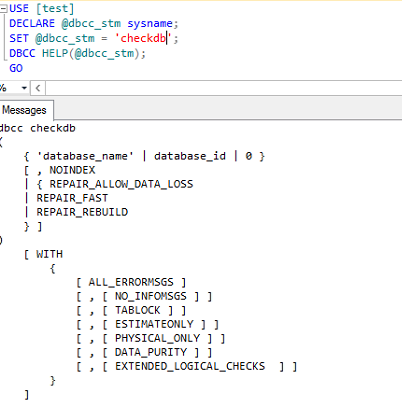
\includegraphics[scale=1]{administration/rep/16}}

\begin{verbatim} database_name | database_id | 0$
\end{verbatim}
Is the name or ID of the database for which to run integrity checks. If not specified, or if 0 is specified, the current database is used. Database names must comply with the rules for identifiers.
\begin{verbatim} NOINDEX
\end{verbatim}
Specifies that intensive checks of nonclustered indexes for user tables should not be performed. This decreases the overall execution time. NOINDEX does not affect system tables because integrity checks are always performed on system table indexes.
\begin{verbatim} REPAIR_ALLOW_DATA_LOSS | REPAIR_FAST | REPAIR_REBUILD
\end{verbatim}
Specifies that DBCC CHECKDB repair the found errors. The specified database must be in single-user mode to use one of the following repair options.
\begin{verbatim} REPAIR_ALLOW_DATA_LOSS
\end{verbatim}
Tries to repair all reported errors. These repairs can cause some data loss.
\begin{verbatim} REPAIR_FAST
\end{verbatim}
Maintains syntax for backward compatibility only. No repair actions are performed.
\begin{verbatim} REPAIR_REBUILD
\end{verbatim}
Performs repairs that have no possibility of data loss. This can include quick repairs, such as repairing missing rows in non-clustered indexes, and more time-consuming repairs, such as rebuilding an index.
\\REPAIR\_REBUILD  does not repair errors involving FILESTREAM data.
\begin{verbatim} ALL_ERRORMSGS
\end{verbatim}
Displays all reported errors per object. All error messages are displayed by default. Specifying or omitting this option has no effect. Error messages are sorted by object ID, except for those messages generated from tempdb database.\\\\
In SQL Server Management Studio, the maximum number of error messages returned is 1000. When you specify ALL\_ERRORMSGS, we recommend that you run the DBCC command by using the sqlcmd utility or by scheduling a SQL Server Agent job to run the command and direct the output to a file. Either of these methods will ensure that running the command once will report all error messages.
\begin{verbatim} EXTENDED_LOGICAL_CHECKS
\end{verbatim}
If the compatibility level is 100 (SQL Server 2008) or higher, performs logical consistency checks on an indexed view, XML indexes, and spatial indexes, where present.\\
For more information, see "Performing Logical Consistency Checks on Indexes," in the "Remarks" section later in this topic.
\begin{verbatim} NO_INFOMSGS
\end{verbatim}
Suppresses all informational messages.
\begin{verbatim} TABLOCK
\end{verbatim}
Causes DBCC CHECKDB to obtain locks instead of using an internal database snapshot. This includes a short-term exclusive (X) lock on the database. TABLOCK will cause DBCC CHECKDB to run faster on a database under heavy load, but decreases the concurrency available on the database while DBCC CHECKDB is running.\\\\
TABLOCK limits the checks that are performed; DBCC CHECKCATALOG is not run on the database, and Service Broker data is not validated.
\begin{verbatim} ESTIMATEONLY
\end{verbatim}
Displays the estimated amount of tempdb space that is required to run DBCC CHECKDB with all the other specified options. The actual database check is not performed.

\begin{verbatim} PHYSICAL_ONLY
\end{verbatim}
Limits the checking to the integrity of the physical structure of the page and record headers and the allocation consistency of the database. This check is designed to provide a small overhead check of the physical consistency of the database, but it can also detect torn pages, checksum failures, and common hardware failures that can compromise a user's data.
\begin{verbatim} DATA_PURITY
\end{verbatim}


Causes DBCC CHECKDB to check the database for column values that are not valid or out-of-range. For example, DBCC CHECKDB detects columns with date and time values that are larger than or less than the acceptable range for the datetime data type; ordecimal or approximate-numeric data type columns with scale or precision values that are not valid.\\\\
Column-value integrity checks are enabled by default and do not require the DATA\_PURITY option. For databases upgraded from earlier versions of SQL Server, column-value checks are not enabled by default until DBCC CHECKDB WITH DATA\_PURITY has been run error free on the database. After this, DBCC CHECKDB checks column-value integrity by default. For more information about how CHECKDB might be affected by upgrading database from earlier versions of SQL Server, see the Remarks section later in this topic.\\\\
If PHYSICAL\_ONLY is specified, column-integrity checks are not performed.\cite{checkdb}


\section{Backups}
Backup is process of an archiving of database content outside of the database. The information is saved in the single or several files which are named backup files. It is possible to restore database form backups to the initial condition. The archiving allows to prevent possibilities of irreversible data loss:
\begin{itemize}
\item media, software or equipment failures 
\item operators errors
\item hackers and virus attacks
\end{itemize}

If backups are stored remotely it also can safe your date in case of natural disasters or other extraordinary circumstances.\\

Previously backups were used to move data to other server, but there is an export command for this case, now. In addition backup can archive data which is not currently useful. 

\subsection{Backup example}
Let's try to study the technique implementation in our database. 
\paragraph{The first step} make a connection with the database, open database folder, click your database by right mouse button, choose Task $\rightarrow $ Back Up.. \\
\centerline{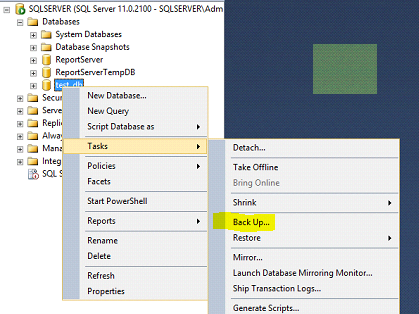
\includegraphics[scale=1]{administration/1}}
\paragraph{The second step} tune general settings:
\begin{itemize}
\item Database - the database which should be archived
\item Backup type - there are different types of backup for example
\begin{itemize}
\item database backup

    A backup of a database. Full database backups represent the whole database at the time the backup finished. Differential database backups contain only changes made to the database since its most recent full database backup.

\item full backup

    A data backup that contains all the data in a specific database or set of filegroups or files, and also enough log to allow for recovering that data.
\item log backup

    A backup of transaction logs that includes all log records that were not backed up in a previous log backup. (full recovery model)
\item file backup

    A backup of one or more database files or filegroups.\cite{backupTypes}
    \\ \\
    In our case we use full one.


\end{itemize}
\item Name - allows to set the name for the backup
\item Description - brief explanation of  backup aims
\item Destination - it is possible to set the address of the backup file and the type of the medium.
\end{itemize}
\centerline{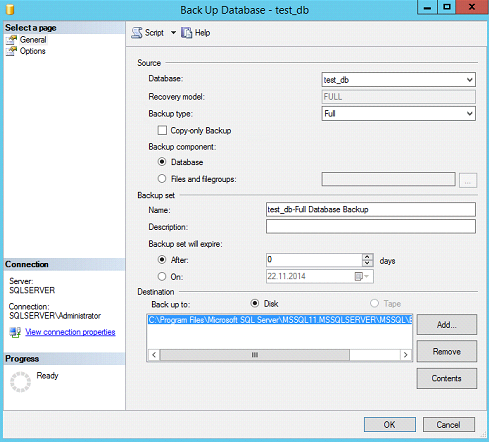
\includegraphics[scale=0.8]{administration/2}}
\paragraph{The third step} Also there are extra settings in an options inset. They can safe storage space and make the backup more reliable.\\\\
\centerline{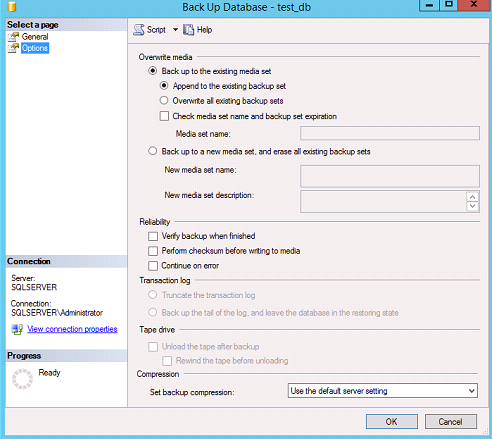
\includegraphics[scale=0.8]{administration/3}}
\paragraph{The fourth step} An operator has to press "OK" button, when all configuration is performed.\\\\
\centerline{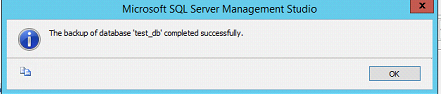
\includegraphics[scale=0.8]{administration/4}}
The backup is finally made.


\subsection{Restore database}
Restore is a process of importing of the backup files inside the database management system. Let's try to restore our database.
\paragraph{The first step} Delete the database form the SQL Server and after that press right mouse button and choose Restore Database form context menu. \\\\
\centerline{
\includegraphics[scale=0.8]{administration/5}}
\paragraph{The second step} In Select Backup Devices press Add.\\\\
\centerline{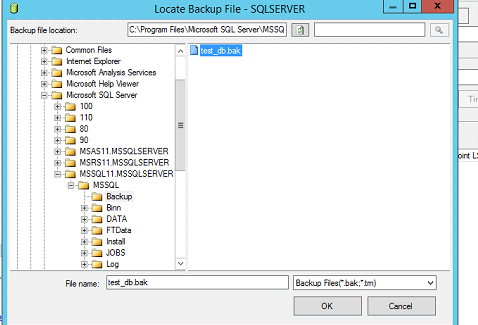
\includegraphics[scale=1]{administration/6}}
\paragraph{The third step} Choose the backup file and press "OK". The file would be added to Backup media field in Select Backup Device window.\\\\
\centerline{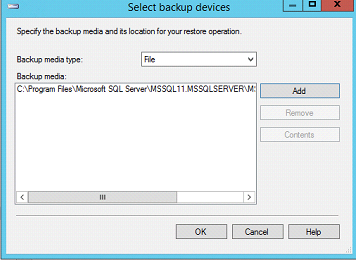
\includegraphics[scale=1]{administration/7}}
\paragraph{The fourth step} Press "OK" again and you will go to the main Restore Database menu and all of the setting would be imported from your backup file. An operator can find files' settings in the files inset, the configuration has same layout as the files configuration during creation of new database.
\\\\
There is also Options part there you can find some advanced settings, for example you can tell the DBMS how it should handle situation if the backup database is same with an exciting one.\\\\
\centerline{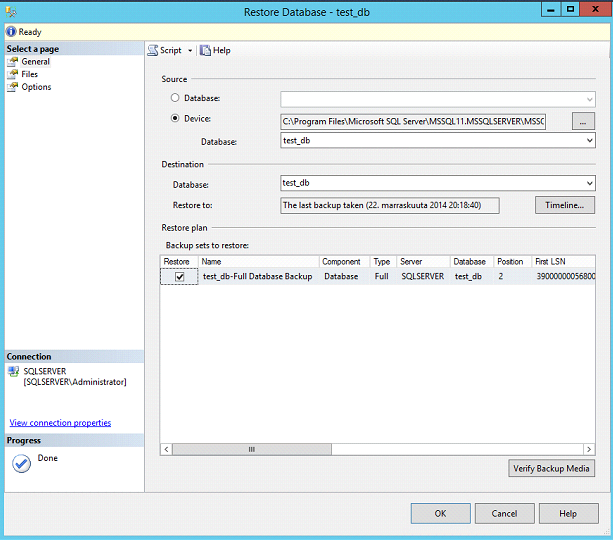
\includegraphics[scale=0.8]{administration/8}}
\centerline{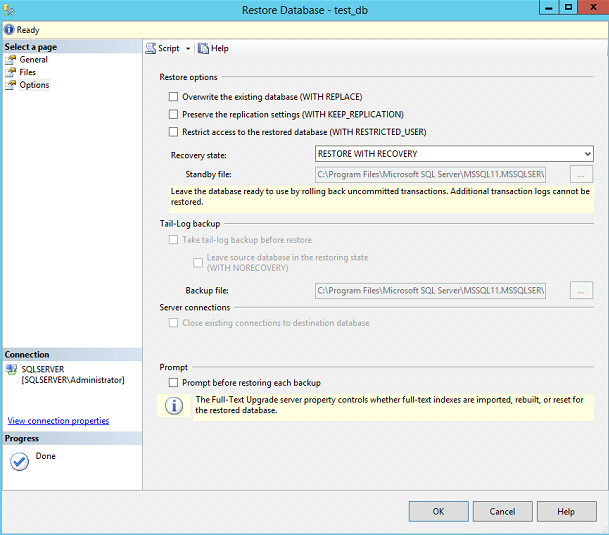
\includegraphics[scale=0.8]{administration/9}}
\paragraph{The firth step} press "OK", if all configurations are perfumed \\\\
\centerline{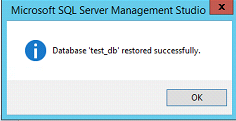
\includegraphics[scale=0.8]{administration/10}}
Our database is restored.\\\\
\centerline{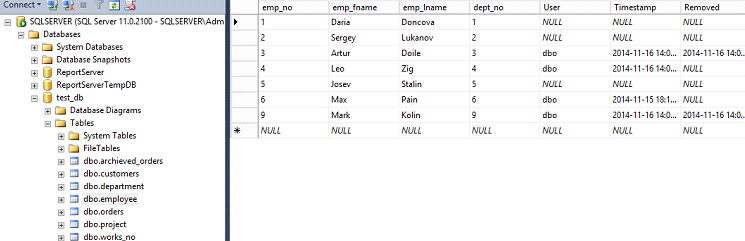
\includegraphics[scale=0.8]{administration/11}}

\subsection{SQL Server Agent}
SQL Server Agent is service that provide different administration tasks in an according with schedule.
\paragraph{The first step} Open SQL Server Configuration choose SQL Server Services, click right mouse button on the SQL Server Agent and press start on the context menu.\\\\
\centerline{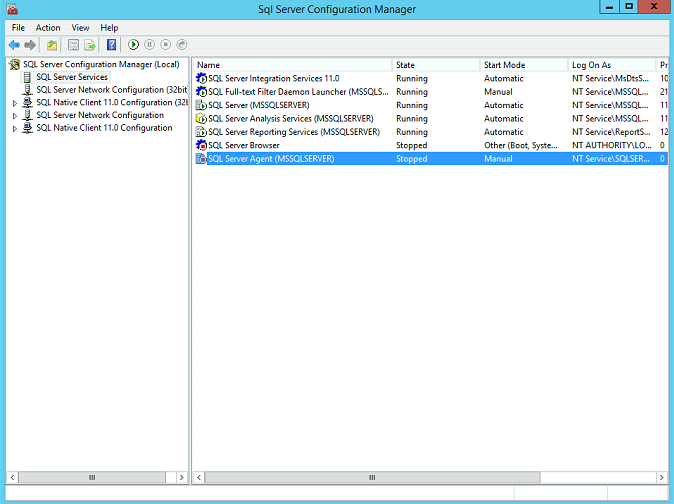
\includegraphics[scale=0.7]{administration/12}}
\paragraph{The second step} Opent SQL Management Studio $\rightarrow $ Management $\rightarrow $ Extended Events $\rightarrow $ click by right mouse button on the Maintenance plane, choose New Maintenance plane.\\\\
\centerline{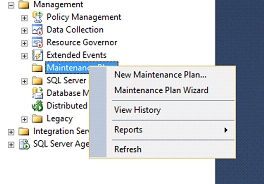
\includegraphics[scale=0.8]{administration/13}}
\paragraph{The third step} Give the name for the plan.\\\\
\centerline{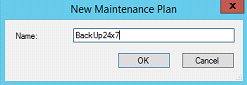
\includegraphics[scale=0.8]{administration/14}}
\paragraph{The fourth} Set the schedule for the maintenance.\\\\
\centerline{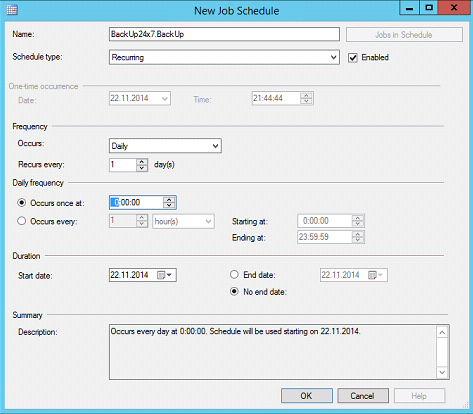
\includegraphics[scale=0.8]{administration/15}}
\paragraph{The firth} Double click the Back Up Database Task option in Toolbox.\\\\
\centerline{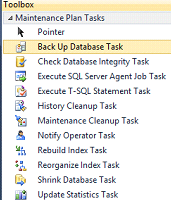
\includegraphics[scale=0.8]{administration/16}}
\paragraph{The sixth step} Double click the icon of Back Up of the design area.\\\\
\centerline{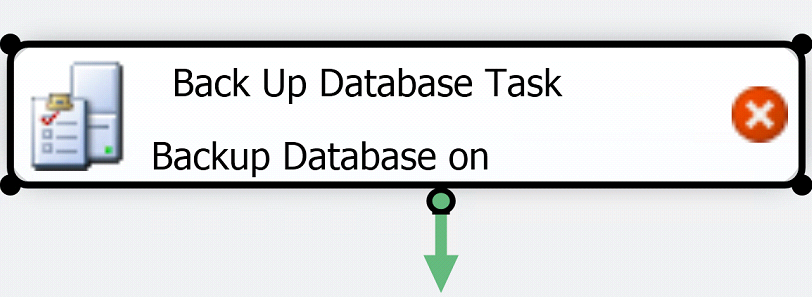
\includegraphics[scale=0.3]{administration/17}}
\paragraph{The seventh step} Set the main backup parameters and press "OK".\\\\
\centerline{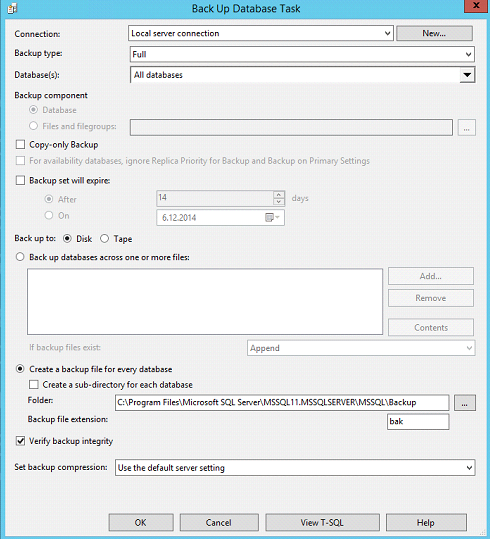
\includegraphics[scale=0.8]{administration/18}}
The maintenance Plan is ready.\\\\
\centerline{
\includegraphics[scale=1]{administration/19}}

\section{Replication}
Replication is a set of processes for copying and sharing data and database objects from one database to another and then synchronizing these databases to maintain consistency. Users, who are connected remotely via Internet, wireless connection, local or wide area networks to the database can get the data, using replication.\cite{repInf}\\\\
Transactional replication mainly used in scenarios that require server-to-server high throughput, which includes:
\begin{itemize}
\item scalability and availability;
\item data warehousing and reporting;
\item integrating data from multiple sires;
\item integrating heterogeneous data;
\item Offloading batch processing.
\end{itemize}
Microsoft SQL Server provides the following types of replication for use in distributed applications \cite{typesRep}:
\begin{itemize}
\item Transactional replication (as soon as the initial snapshot is taken, subsequent data changes and schema modifications made at the Publisher are usually delivered to the Subscriber as they occur (in near real time). The data changes are applied to the Subscriber in the same order and within the same transaction boundaries as they occurred at the Publisher) \cite{transRep}.

\item Merge replication (Subsequent data changes and schema modifications made at the Publisher and Subscribers are tracked with triggers. The Subscriber synchronizes with the Publisher when connected to the network and exchanges all rows that have changed between the Publisher and Subscriber since the last time synchronization occurred) \cite{mergRep}.

\item Snapshot replication (distributes data exactly as it appears at a specific moment in time and does not monitor for updates to the data. When synchronization occurs, the entire snapshot is generated and sent to Subscribers) \cite{snapRep}.
\end{itemize}
The type of replication you choose for an application depends on many factors, including the physical replication environment, the type and quantity of data to be replicated, and whether the data is updated at the Subscriber \cite{typesRep}.\\\\
Each type of replication typically begins with an initial synchronization of the published objects between the Publisher and Subscribers. This initial synchronization can be performed by replication with a snapshot, which is a copy of all of the objects and data specified by a publication. After the snapshot is created, it is delivered to the Subscribers. For some applications, snapshot replication is all that is required. For other types of applications, it is important that subsequent data changes flow to the Subscriber incrementally over time. Some applications also require that changes flow from the Subscriber back to the Publisher. Transactional replication and merge replication provide options for these types of applications.
\subsection{Replication Creation}
\begin{figure}[H]
\centerline{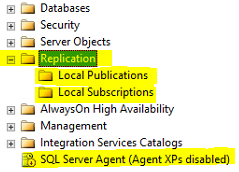
\includegraphics[scale=1]{administration/rep/1}}
\caption{Replication of a database. Transaction distribution is off.}
\end{figure}
Replication makes copies and share them from the Publisher database to the Subscriber. If there will be some changes in the copy of one object, the changes can effect on others. As you can see in the Figure 2, a Distributor can be used by other Publisher, also Publisher can act as its own Distributor and Server can be a Publisher that uses another server as a Distributor.\\\\

Basically, we have Publishers databases and Subscribers databases. First one publish and share their data, others get their data. Like in a social sites or news sites, someone shares the news, he is a publisher, and others, who liked this post and subscribed that, they are subscribers.
\begin{figure}[H]
\centerline{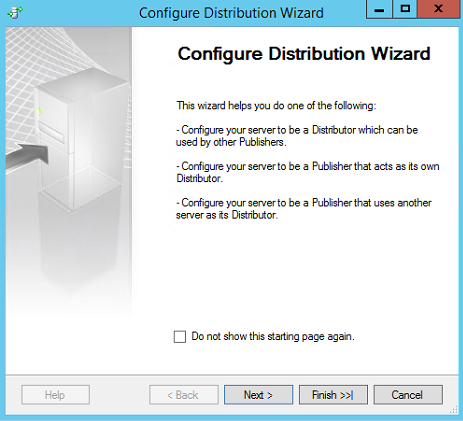
\includegraphics[scale=0.9]{administration/rep/2}}
\caption{Configuration of a replication. Making our database a distributor or publisher.}
\end{figure}

\begin{figure}[H]
\centerline{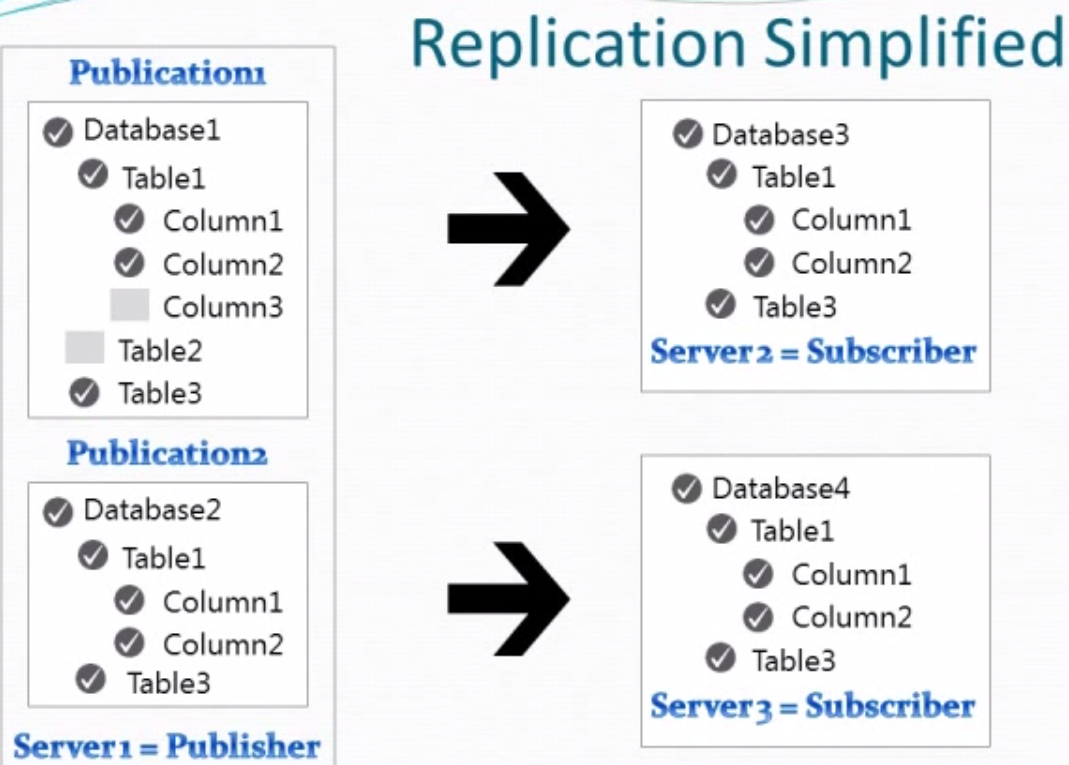
\includegraphics[scale=0.5]{administration/rep/3}}
\caption{Basic diagram of a replication.}
\end{figure}

You can publish:
\begin{itemize}
\item Tables
\item Stored Procedures
\item User Defined Functions
\item Views
\item Indexed Views (as a Table)
\item Indexed Views (Definition)
\item DDL Commands
\end{itemize}

\begin{figure}[H]
\centerline{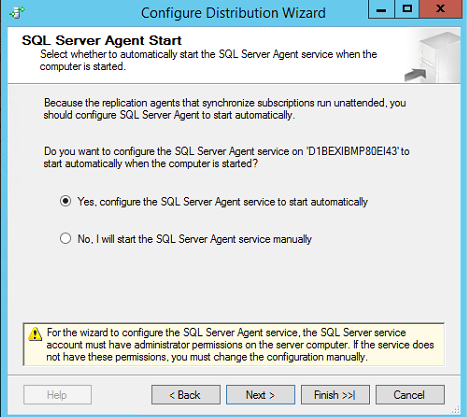
\includegraphics[scale=1]{administration/rep/4}}
\caption{Select starting SQL Server Agent undisabled.}
\end{figure}

\begin{figure}[H]
\centerline{
\includegraphics[scale=0.8]{administration/rep/5}}
\caption{Snapshot replication location.}
\end{figure}

\begin{figure}[H]
\centerline{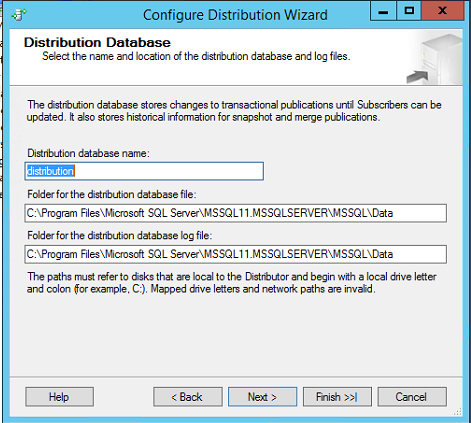
\includegraphics[scale=0.8]{administration/rep/6}}
\caption{ Distribution database.}
\end{figure}

\begin{figure}[H]
\centerline{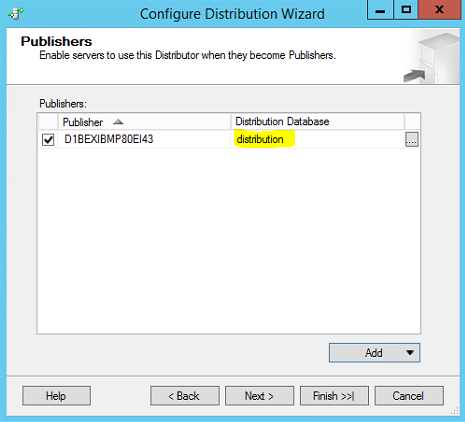
\includegraphics[scale=0.8]{administration/rep/7}}
\caption{The list of publishers}
\end{figure}

\begin{figure}[H]
\centerline{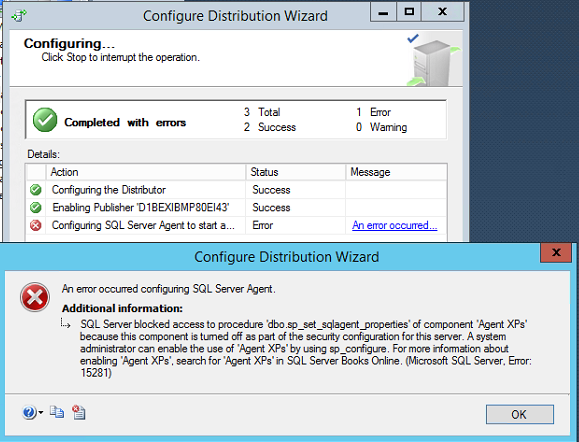
\includegraphics[scale=0.8]{administration/rep/8}}
\caption{Agent did not start automatically, we have to start it manually}
\end{figure}

\begin{figure}[H]
\centerline{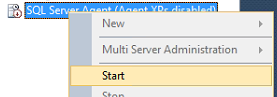
\includegraphics[scale=0.8]{administration/rep/9}}
\caption{Starting manually}
\end{figure}

\begin{figure}[H]
\centerline{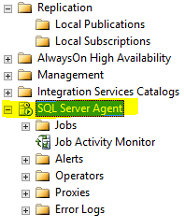
\includegraphics[scale=0.8]{administration/rep/10}}
\caption{Server manager starts}
\end{figure}

\begin{figure}[H]
\centerline{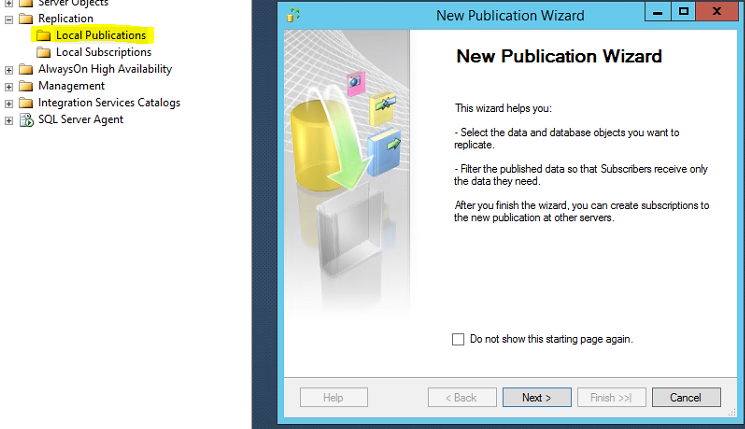
\includegraphics[scale=0.8]{administration/rep/11}}
\caption{Create a Publication.}
\end{figure}
Right now we will create a Publication that means we will select what the Data will be replicated, distributed. \\\\
\begin{figure}[H]
\centerline{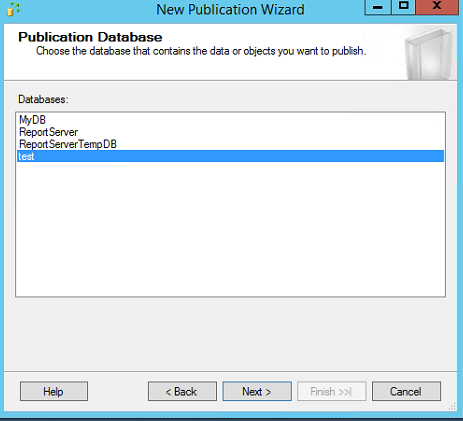
\includegraphics[scale=0.82]{administration/rep/12}}
\caption{What database will be replicated?}
\end{figure}

\begin{figure}[H]
\centerline{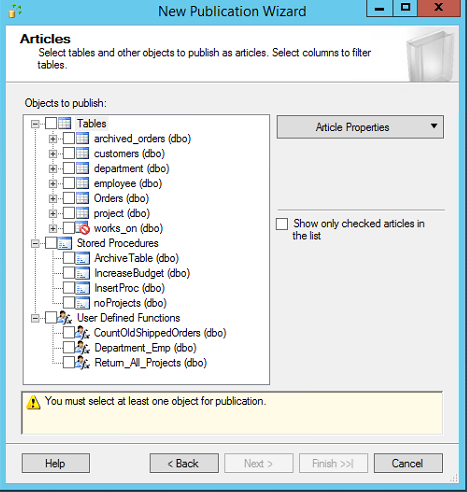
\includegraphics[scale=0.82]{administration/rep/13}}
\caption{Selecting the data to publish}
\end{figure}
So, I have created a Transaction Replication as an example. And each user or server, who login to my server can work and see my publication. It is common now.

\begin{figure}[H]
\centerline{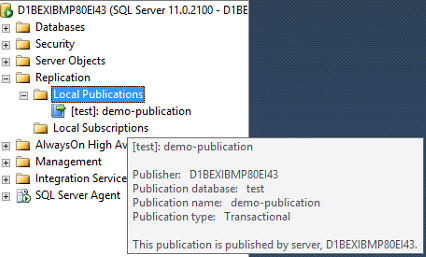
\includegraphics[scale=0.8]{administration/rep/14}}
\caption{ Replication Created}
\end{figure}
\newpage
\begin{thebibliography}{@@@@}
\bibitem{sysdb}
			\href{http://msdn.microsoft.com/en-us/library/ms178028.aspx }{MSDN - System database SQL server and files}
 (\today)
\bibitem{checkdb}
			\href{http://msdn.microsoft.com/en-us/library/ms176064.aspx  }{MSDN - CHECKDB}  (\today)	
	\bibitem{backupTypes}
			\href{http://msdn.microsoft.com/en-us/library/ms175477.aspx}{MSDN - Backup Overview}  (\today)	
	\bibitem{repInf}
			\href{http://msdn.microsoft.com/en-us/library/ms151198(v=sql.110).aspx}{MSDN -  Replication basic information}  (\today)
			
	\bibitem{typesRep}
			\href{http://msdn.microsoft.com/en-us/library/ms152531(v=sql.110).aspx}{MSDN - Types of replications}  (\today)
			\bibitem{transRep}
			\href{http://msdn.microsoft.com/en-us/library/ms151176(v=sql.110).aspx}{MSDN -   Transactional replication}  (\today)
	\bibitem{mergRep}
			\href{http://msdn.microsoft.com/en-us/library/ms152746(v=sql.110).aspx}{MSDN -  Merge replication}  (\today)
	\bibitem{snapRep}
			\href{http://msdn.microsoft.com/en-us/library/ms152746(v=sql.110).aspx  }{MSDN -Snapshot replication}  (\today)

				

	\end{thebibliography}
	


\end{document}
